\chapter{Induction}

\textit{I was at first almost frightened when I saw such mathematical force made to bear upon the subject, and then wondered to see that the subject stood it so well.}\\
\noindent\textbf{-   Michael Faraday}

\vspace{1cm}


\begin{marginfigure}%
  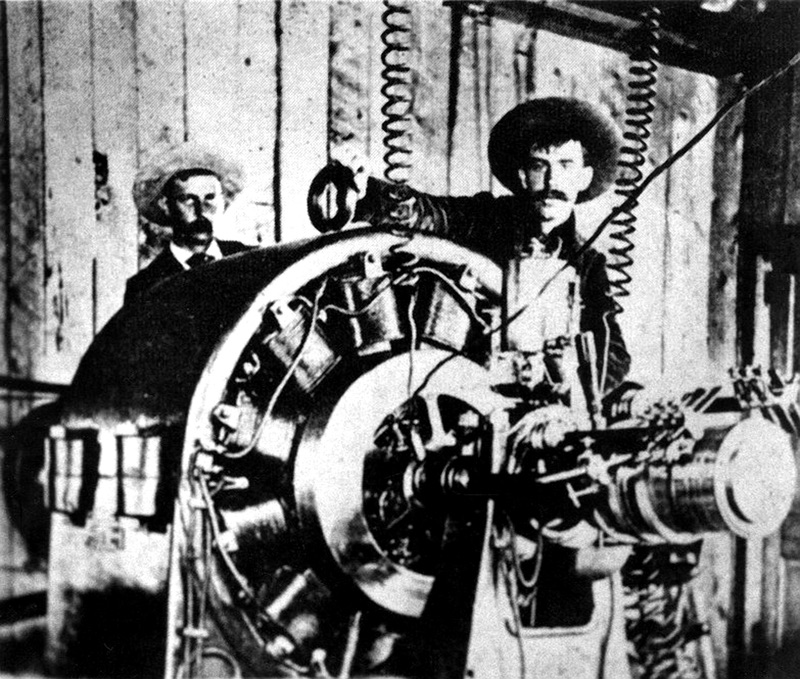
\includegraphics[width=\linewidth]{generator.jpg}
  \caption{Dudes posing with their Westinghouse alternator in 1891}
  \label{fig:marginfig}
\end{marginfigure}


\marginnote[20pt]{
\section{Magnetic Flux}
Magnetic flux $\Phi_B$ is the is the sum of magnetic field $\overrightarrow{B}$ passing through a surface area $\overrightarrow{A}$.
$$ \Phi_B=\sum\overrightarrow{B}\cdot \Delta\overrightarrow{A}$$ }


\begin{marginfigure}[20pt]%
  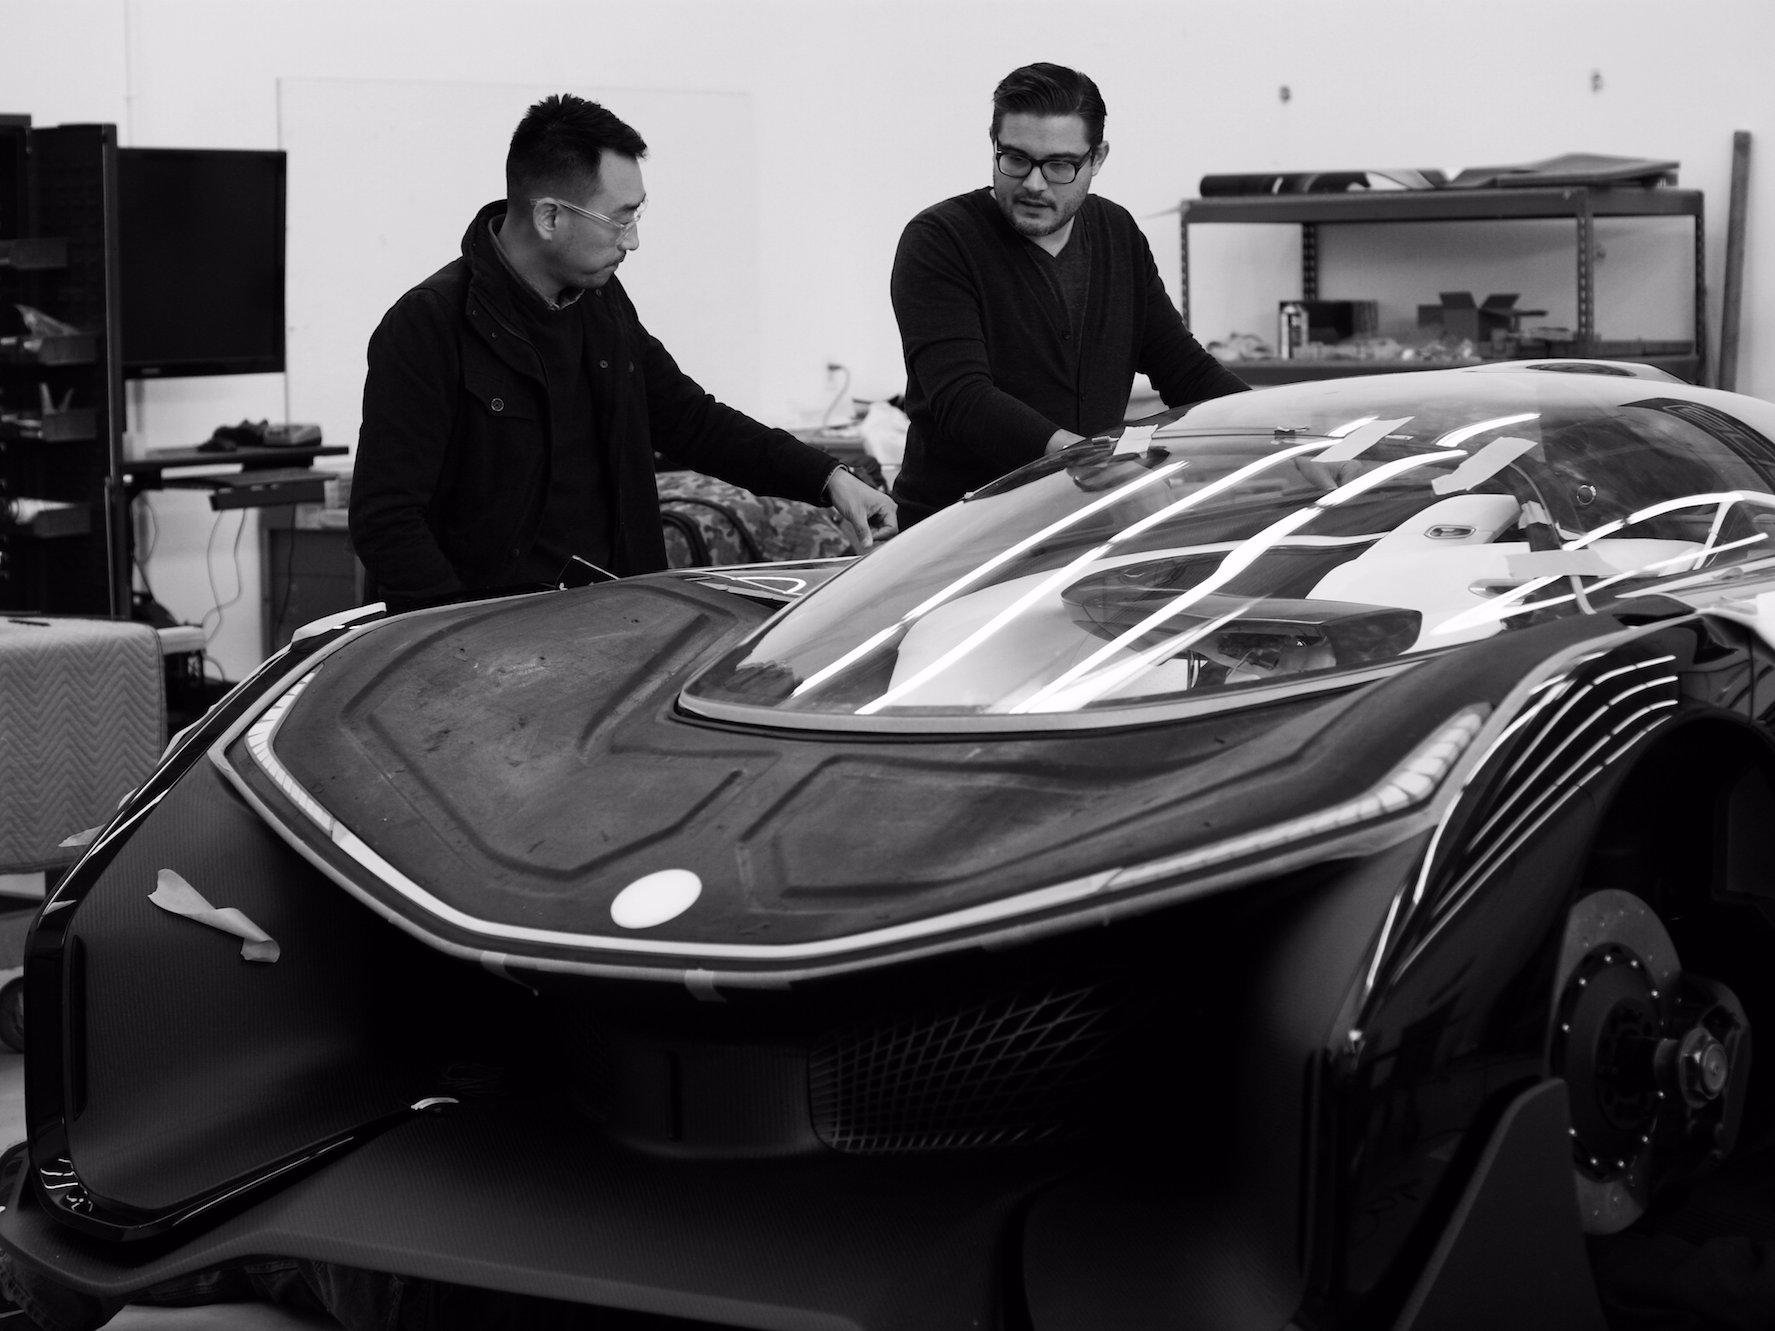
\includegraphics[width=\linewidth]{ffzero.jpg}
  \caption{\textit{Faraday Future} engineers prototyping the FFZERO in 2016  }
  \label{fig:marginfig}
\end{marginfigure}


\section{Electromotive Force}
Electromotive force, or emf, is denoted $\mathcal{E} $.  It is the voltage developed through a conducting circuit by a battery or dynamo.  It is not a force but an integral of the electric field over the current path.  It is similar to a voltage difference but may be non-zero over a closed path. 

\section{Motional Emf}
Consider a conducting bar of length $l$ moving perpendicularly through a magnetic field.  The charge carriers in the conductor undergo a magnetic force.  

$$\overrightarrow{F}_{B}=q\overrightarrow{v}\times \overrightarrow{B}$$

The conductor will polarize as the charge carriers move up until the point equilibrium is reached.  The effect is that an electric potential difference is maintained between the ends of a conductor moved perpendicularly through a magnetic field.  To determine the magnitude of this potential begin by equating the magnetic force and the electrostatic force.
$$F_E=F_B$$
$$qE=qvB \hspace{2cm} E=vB$$
Once the strength of the electric field is determined a potential difference is derived.
$$\Delta V=El=Blv$$

\newpage
\begin{marginfigure}[10pt]%
  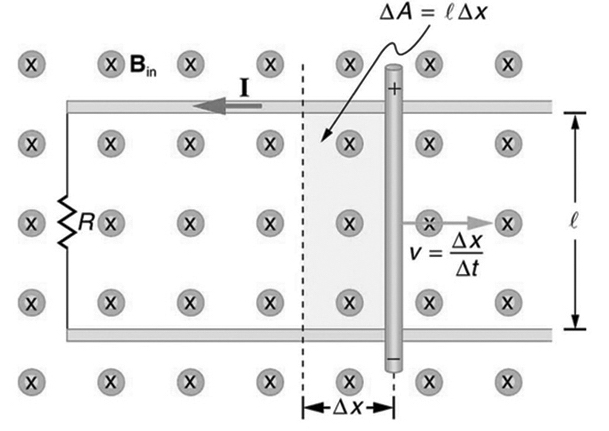
\includegraphics[width=\linewidth]{motional.jpeg}
  \caption{Motional emf}
  \label{fig:marginfig}
\end{marginfigure}
\noindent Now consider when the conducting bar is made part of a closed circuit with resistance $R$. In this case charge is free to flow through the circuit.  The bar is at position $x$.  The magnetic flux is determined as follows.
$$\Phi_B=Blx$$
The motional emf is determined.  
$$ \mathcal{E}=-\frac{d\Phi_B}{dt}=-Blv$$



\subsection{Power}
The power dissipated by the circuit is determined as follows.  Find the mechanical power.
$$P=Fv=IlBv=\frac{B^2l^2v^2}{R}$$
Find the electrical power. 
$$P=\frac{V^2}{R}=\frac{\mathcal{E}^2}{R}=\frac{B^2l^2v^2}{R}$$
Note their equivalence.


\section{Faraday's Law}
\begin{marginfigure}[150pt]%
  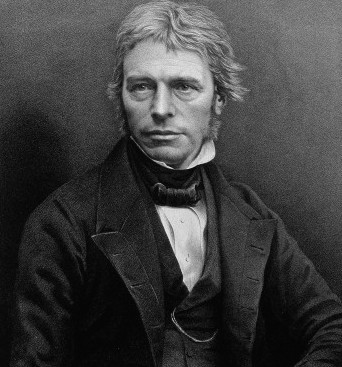
\includegraphics[width=\linewidth]{faraday.jpg}
  \caption{Michael Faraday}
  \label{fig:marginfig}
\end{marginfigure}

An emf is induced in a circuit by a changing magnetic field either by changing the area, relative orientation or strength of the magnetic field.  The induced emf is directly proportional to the time rate of change of the magnetic flux through the circuit.
$$ \mathcal{E}=-\frac{\Delta\Phi_B}{\Delta t} \hspace{2cm} \Phi_B=\sum\overrightarrow{B}\cdot \Delta\overrightarrow{A}$$
And for a circuit with $N$ coil loops.
$$ \mathcal{E}=-N\frac{\Delta\Phi_B}{\Delta t}$$



\section{Lenz's Law}
The induced emf produces a current which creates magnetic flux opposite the change of magnetic flux through the loop.\\ 

There are many ways to do this bookkeeping.  One way is to use a left hand rule.

\section{Induced Emf and Electric Field}
An electric field is generated in the conductor as a result of the changing magnetic flux.  In fact, an electric field is always generated by a changing magnetic flux, even in free space.
$$\sum_{\text{\tiny boundary}}\overrightarrow{E}\cdot \Delta\overrightarrow{s}=-\frac{\Delta\Phi_B}{\Delta t}$$


\section{Inductance}
\marginnote[-30pt]{
\subsection{Unit}
The unit for inductance is the Henry.  It is defined as the Volt second per Ampere.
$$1 \ \text{Henry}=\frac{1\ \text{Volt second}}{1\ \text{Ampere}}$$}
The term inductance was coined by Oliver Heaviside in 1886.  It is the property of an electrical conductor by which a change in current flowing through it induces an electromotive force in both the conductor itself (self-inductance) and in nearby conductors (mutual inductance).
$$ \mathcal{E}_L=-N\frac{\Delta\Phi_B}{\Delta t}=-L\frac{\Delta I}{\Delta t}$$
$$L=\frac{N\Phi_B}{I}$$



\section{RL Circuits}
\marginnote[0pt]{A simple RL circuit consists of a resistor and inductor in series with a battery.  The example circuit has a open switch that is closed at time $t=0$.  The resulting current approaches a constant value asymptotically.\\
Without the battery the circuit may be perturbed by giving the inductor a pulse of magnetic field.  In this case the current will decay exponentially.}
$$\begin{circuitikz} 
\draw
(0,0) to[battery] (4,0) to[closing switch] (4,2)
      to[resistor, l=$R$] (2,2) to[inductor, l=$L$] (0,2) -- (0,0);
\end{circuitikz}
$$
$$ \mathcal{E}=IR+L\frac{\Delta I}{\Delta t}$$
$$I(t)=\frac{\mathcal{E}}{R}\left(1-e^{-\frac{R}{L}t}\right)$$
%\vspace{1cm}

\section{LC Circuits}
\marginnote[0pt]{A simple LC circuit consists of a capacitor and inductor in series.  The example circuit begins with the capacitor charged and has a open switch that is closed at time $t=0$.  The resulting current is a sinusoidal oscillation.\\
Without the capacitor initially charged the circuit may be perturbed by giving the inductor a pulse of magnetic field.}
$$\begin{circuitikz} 
\draw
(0,0) -- (4,0) to[closing switch] (4,2)
      to[capacitor, l=$C$] (2,2) to[inductor, l=$L$] (0,2) -- (0,0);
\end{circuitikz}
$$
$$ 0=\frac{Q}{C}+L\frac{\Delta I}{\Delta t}$$
$$Q(t)=Q_0 \cos\left(\frac{t}{\sqrt{LC}}\right)$$
$$I(t)=-\frac{Q_0}{\sqrt{LC}} \sin\left(\frac{t}{\sqrt{LC}}\right)$$
%\vspace{1cm}
\section{Inductor Energy}
Consider the power dissipated in a RL circuit.
$$P=I \mathcal{E}=I^2R+LI\frac{\Delta I}{\Delta t}$$
The term representing the rate of change of energy stored in the magnetic field is shown below. 
$$\frac{\Delta U_B}{\Delta t}=LI\frac{\Delta I}{\Delta t}$$
The energy stored in the magnetic field is written as follows.
$$U_B=\frac{LI^2}{2}$$


\section{Maxwell's Equations}

\vspace{1cm}
\subsection{Gauss's Law}

$$\sum_{\text{\tiny boundary}}\overrightarrow{E}\cdot \Delta\overrightarrow{A}=\frac{q_{enc}}{\epsilon_0}$$

\vspace{1cm}
\subsection{Gauss's Law for Magnetism}

$$\sum_{\text{\tiny boundary}}\overrightarrow{B}\cdot \Delta\overrightarrow{A}=0$$

\vspace{1cm}
\subsection{Ampere-Maxwell Law}

$$\sum_{\text{\tiny boundary}}\overrightarrow{B}\cdot \Delta\overrightarrow{s}=\mu_0 I+\mu_0\epsilon_0\frac{\Delta\Phi_E}{\Delta t}$$

\vspace{1cm}
\subsection{Faraday's Law}

$$\sum_{\text{\tiny boundary}}\overrightarrow{E}\cdot \Delta\overrightarrow{s}=-\frac{\Delta\Phi_B}{\Delta t}$$